\chapter{Algorithmical Design}
  Calculating a solution for a specific scenario is split into two parts. At first the underlying connection topology is determined.
  Subsequently a channel assignment is computed for this specific topology. As input we expect a connected, undirected, weigthed graph.
  Note that this chapter and algorithms only deal with graphs and the computation of solutions on graphs.
  
  \begin{figure}[htbp]
    \centering
    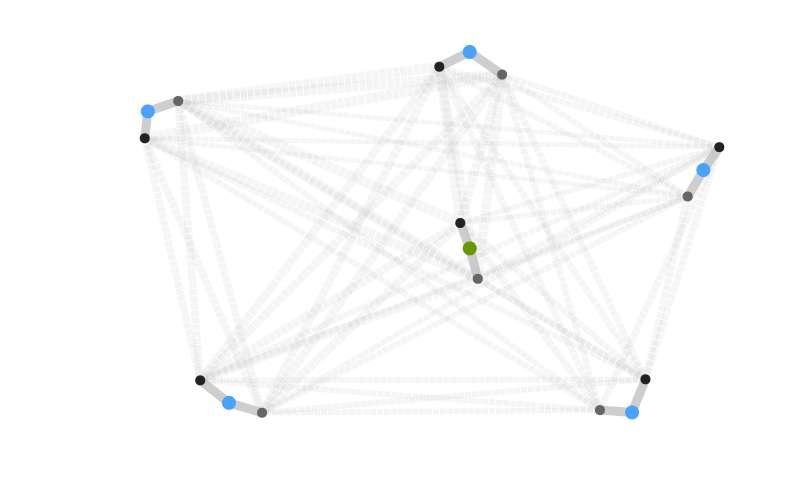
\includegraphics[width=1\columnwidth]{figures/graphseen.png}
    \caption{Graph representation of a scenario with 6 APs and 2 modules each. The grey eges indicate possible connectivity between the 
      modules. Edge weight(SNR) is mapped to edge thickness.}
    \label{fig:graphseen}
  \end{figure}
  
  \section{Topology Creation}
    Creating the topology is split into two parts. 
    First creating the minimal spanning tree with respect the provided formula.
    And second adding redundancies in form ofbackup or parallel links to the \ac{MST}.    

    \subsection{Minimal/Optimal Spanning Tree Topology}
      \subsubsection{Description}
	In order to select those edges we want to use for creating connections between the APs, we use a derivation of the \ac{DJP} algorithm \cite{prim}\cite{jarnik}.
	The reason we chose a \ac{MST} algorithm over other techniques like all-pairs shortest path is, that a MST gives us the best essential edges in a graph. 
	This essential set of edges we can then extend by additional edges if we have or want to (survival paths). 
	Chosing more than the essential edges in the beginning would immeadiatly play in favor of interference, which we want to avoid by all means.      
	
	We start by selecting an arbitray initial node and marking it as visited. All edges from this set of visited nodes to unvisited nodes are called productive edges.
	We keep those productive edges in a list sorted by their scores. The score of an edge is determined by the following formula:
	
	\begin{equation} \label{eq:edgescore}
	  ES=\frac{b}{(i + 1 )* (c + 1)}
	\end{equation}
	
	where \textit{ES} is the Score of this Edge, \textit{b} is the expected bandwidth, \textit{i} is the number of 
	interfering modules and \textit{c} is the connected count of the corresponding nodes.
	
	For each round we determine from this list the edge with the highest score. If we encounter a tie in scores, 
	we chose those edges which have the highest SNR value and as a last
	resort we pick one at random. We then mark the new node as visited and add also the new links to the list.
	Finally we have to update the scores for each affected link and continue with the next round until all nodes are marked visited.
	The outcome is a minimal spanning tree for this graph with a custom evaluation function.
	
	\newpage
	
	\begin{description}
	  \item[Expected Bandwidth]
	    describes the expected available bandwidth we assume to get for this link depending on the Signal-to-Noise-Ratio.
	    For a given Signal-to-Noise-Ratio we can estimate the maximal possible thoughput.
	    The bandwidth was chosen as the numerator, since it is effectively shared by the radio modules within range.
	    As we can see from the diagram, a higher SNR value results in more bandwidth available and works in favor of this edge.
	    Note that the mapping of SNR to achievable throughput may have to be adjusted for different hardware/devices. 
	    In general the behaviour will stay the same, as a higher SNR will necessarily result in a better modulation, which
	    also increases throughput.
	  
	  \item[Connected Count]
	    Number of nodes we can reach from Module A and Module B by just using module-module edges. 
	    A higher connected count diminishes the importance of this edge, since this value controls how many channels we can use later for the overall graph.
	    If this value would not be taken into consideration for calculating the score, the algorithm would rather create long chains of connected modules. 
	    Those links in this chain would admittedly have the best SNR values, but since they have to share the same channel, it would result in lowering the overall throughput.
	    Granting this value a higher impact in the formula, like for example in 
	    
	    \begin{equation}
	      ES=\frac{b}{(i + 1)* (c + 1)^2}
	    \end{equation}
	    
	    , would have the effect of overemphasizing 
	    the channel distribution and lead to poor choices in links with respect to SNR - lowering overall throughput again.
	    The simple, linear impact in the formula has been shown to achieve the best tradeoff between those two extremes.
	    
	  \item[Interfering Modules]
	    Since the channel assignment has not taken place yet, we do not know which modules are actually interfering with this link if we would use it.
	    However we do know to which other modules this module already has connections to and since those have to use the same channel in order to communicate with each
	    other, we can derive an estimate as lower bound for the number of interfering modules for this link (A,B) by counting the following modules:
	    Total Interfering Modules = Number of visited nodes which we can reach by one hop over a module-module connection from node A and B.
	    Those modules definetly interfer with our current connection, since they:
	    
	    \begin{itemize}
	    \item are in range with at least one node of this connection (one hop distance)
	    
	    \item have to use the same channel (communication over module-module link)
	    
	    \item do actually interfere, because we already decided to use this connection (visited node)
	    \end{itemize}

	    The value is incremented by one, because if this connection would be used, itself again acts as a source for interference.
	    With an increasing count in interfering modues, the value of the link decreases and vice versa. This reflects perfectly the concept of a shared medium.
	\end{description}
\newpage
	\begin{figure}[h!]
	  \centering
	  \includegraphics[width=0.6\columnwidth]{figures/snr_tp}
	  \caption{Expected throughput \ac{SNR}-values by \cite{expected_snr}. We assume to get the best possible throughput for a given SNR, since 
	    modulation is automatically adapted by the APs with increasing SNR.}
	  \label{fig:snr_tp}
	\end{figure}

	\begin{figure}[h!]
	  \centering
	  \includegraphics[width=1\columnwidth]{figures/formula_graphic}
	  \caption{Impact of the connected count on the formula. Resulting topology in case the connected count is underemphasized (left) leading
	    to long chains of possibly high quality links, but only one useable channel, which has to be shared among all modules.
	    Topology in case of an overemphasized connected count (right). As the algorithm avoids reutilizing already used modules,
	    links with low quality are preferred, leading a lot of exclusive channels with lower link quality.}
	  \label{fig:formula_graphic}
      \end{figure}
\newpage
	
      \subsubsection{Example}
	Let's take a look at a simplified example, where we assume \textit{b=SNR}. Also note that we immediately expand module-device edges to keep the example short.
	Normally the algorithm would also expand each of those edges step by step. However due to their maximum weight these have precedence over all other edges, 
	so that we merely skip a few images.
      \begin{figure}[h!]
	\begin{minipage}{0.5\textwidth}
	  \includegraphics[width=\columnwidth]{figures/mst_calc_1}
	\end{minipage}
	\caption{Example input topology. The edge-weights here represent the SNR value.}
	\label{fig:mst_calc_initial}
      \end{figure}      
      \begin{figure}[h!]
	\centering
	\begin{minipage}{0.4\textwidth}
	  \includegraphics[width=\textwidth]{figures/mst_calc_2}
	\end{minipage}
	\qquad
	\begin{minipage}{0.49\textwidth}
	  \begin{tabular}{c||c|c|c||c}
	    Edge & \textit{b} & \textit{i} & \textit{c} & \textit{ES}\\ \hline\hline
	    (A,D) & 40 & 0 & 0 & 40 \\ \hline
	    \textbf{(C,D)} & \textbf{90} & \textbf{0} & \textbf{0} & \textbf{90} \\ \hline
	    (A,P) & 12 & 0 & 0 & 12 \\ \hline
	    (C,D) & 30 & 0 & 0 & 30 \\ \hline
	  \end{tabular}
	\end{minipage}
	\caption{First round. Picking (C,D) with highest score.}
	\label{fig:mst_calc_2}
      \end{figure}
      \begin{figure}[h!]
	\centering
	\begin{minipage}{0.5\textwidth}
	  \includegraphics[width=\columnwidth]{figures/mst_calc_3}
	\end{minipage}
	\begin{minipage}{0.35\textwidth}
	  \begin{tabular}{c||c|c|c||c}
	    Edge & \textit{b} & \textit{i} & \textit{c} & \textit{ES}\\ \hline\hline
	    (A,P) & 12 & 0 & 0 & 12 \\ \hline
	    (C,P) & 30 & 1 & 1 & 7.5 \\ \hline
	    (G,P) & 50 & 0 & 0 & 50 \\ \hline
	    (G,N) & 96 & 0 & 0 & 96 \\ \hline
	    \textbf{(G,K)} & \textbf{97} & \textbf{0} & \textbf{0} & \textbf{97} \\ \hline
	    (G,H) & 22 & 0 & 0 & 22 \\ \hline
	    (E,H) & 23 & 0 & 0 & 23 \\ \hline
	  \end{tabular}
	\end{minipage}
	\caption{Second round. Score for edge (C,P) was decreased, since Module D is used once. Picking edge (G,K).}
	\label{fig:mst_calc_3}
      \end{figure}
      
      \newpage
      
      \begin{figure}[h!]
	\centering
	\begin{minipage}{0.5\textwidth}
	  \includegraphics[width=\columnwidth]{figures/mst_calc_4}
	\end{minipage}
	\begin{minipage}{0.49\textwidth}
	  \begin{tabular}{c||c|c|c||c}
	    Edge & \textit{b} & \textit{i} & \textit{c} & \textit{ES}\\ \hline\hline
	    (A,P) & 12 & 0 & 0 & 12 \\ \hline
	    (C,P) & 30 & 1 & 1 & 7.5 \\ \hline
	    (G,P) & 50 & 1 & 1 & 12.5 \\ \hline
	    \textbf{(G,N)} & \textbf{96} & \textbf{1} & \textbf{1} & \textbf{24} \\ \hline
	    (G,H) & 22 & 1 & 1 & 5.5 \\ \hline
	    (E,H) & 23 & 0 & 0 & 23 \\ \hline
	    (K,J) & 20 & 1 & 1 & 5 \\ \hline
	    (M,N) & 23 & 0 & 0 & 23 \\ \hline
	  \end{tabular}
	\end{minipage}
	\caption{Third round. All edges connected to G have been recalculated. Best edge is (G,N).}
	\label{fig:mst_calc_4}
      \end{figure}
      
      \begin{figure}[h!]
	\centering
	\begin{minipage}{0.5\textwidth}
	  \includegraphics[width=\columnwidth]{figures/mst_calc_5}
	\end{minipage}
	\begin{minipage}{0.49\textwidth}
	  \begin{tabular}{c||c|c|c||c}
	    Edge & \textit{b} & \textit{i} & \textit{c} & \textit{ES}\\ \hline\hline
	    \textbf{(E,H)} & \textbf{23} & \textbf{0} & \textbf{0} & \textbf{23} \\ \hline
	    (G,H) & 22 & 2 & 2 & 2.4 \\ \hline
	    (K,J) & 20 & 1 & 2 & 3.3 \\ \hline
	  \end{tabular}
	\end{minipage}
	\caption{Fourth and final round. Edgescores of the remaining links rapidly decrease as using those would definetly cause interference. 
	  Best edge to connect the last nodes is (E,H)}
	\label{fig:mst_calc_5}
      \end{figure} 
      \begin{figure}[h!]
	\begin{minipage}{0.5\textwidth}
	  \includegraphics[width=\columnwidth]{figures/mst_calc_6}
	\end{minipage}
	\caption{Resulting MST}
	\label{fig:mst_calc_6}
      \end{figure}  
     \newpage
      
    \subsection{Survival Path}
      A spanning tree is very susceptible to graph partition by just removing or failing one link so we have to add redundancies in form of supplementary connections.
      However those redundant connections have to be carefully chosen in order not to negatively impact the successive channel assignment and neither to push interference.
      Note that this is an optional feature, since for some usecases a spanning tree topology is enough or a topology with redundand links is not easily implemented.  
      
      We accomplish this by iterating over all the edges of the spanning tree and simulate each connection failing. We then check if there still exists 
      a path from Node A to Node B of this failing connection. Only if this failing connection cuts the graph in half and there is no path to the other side,
      we start looking for a backup route in the following fashion:
      First we separate the the graph into two groups: Group A with all nodes and links reachable from Node A and Group B the same for Node B.
      We create a list with unused edges which connect the two groups and calculate the scores on them and pick again the edge with the highest score.
      This edge is, considering to the formula, the best edge to reconnect the two parts is called the survival edge for this scenario.
      Nevertheless we have to be aware that it might not be feasible to reconnect those parts if the underlying structure does not permit it.
      For example if the link between nodes \(E\) and \(F\) in \ref{fig:survival_algo} might be the only connection possible and failing it would cause network disruption.
      This results in a robust network topology, which despite the added interfering links still yields a high overall throughput with redundant paths.
      The survival path attribute for a graph can be expressed in the following way:
      \begin{quote}
	For each edge (a,b) of the calculated spanning tree graph G', find a path from a to b without traversing (a,b), 
	in a way that the the sum of the Edgescores of the path is maximal.
      \end{quote}
      Formal description:
      $$\textit{G}=(\textit{V},\textit{E}) \quad
	\forall \textit{edge}_\textit{a,b} \exists \textit{path}_\textit{a,b} | \textit{edge}_\textit{a,b} \notin \textit{path}_\textit{a,b} \quad
	\textit{a,b} \in \textit{V}, \textit{edge}_\textit{a,b} \in \textit{E}$$
	Finding the optimal edge:
	$$\textit{max}(\textit{edgescore}(\textit{path}_\textit{a,b})) |
	\textit{edgescore}(\textit{path}_\textit{a,b})) = \sum_{\substack{e \in \textit{path}_\textit{a,b}}} \textit{edgescore}(e)$$
      \begin{figure}[h!]
	\centering
	\includegraphics[width=1\columnwidth]{figures/survival_algo2}
	\caption{Finding survival paths. Simulation of connection between node A and node B failing, creating two groups.
	  Finding a survival path for node A and B. Eventually all connections have a survival path. Here no redundant link possible for failing connection E,F.}
	\label{fig:survival_algo}
      \end{figure}
      
     \newpage

  \section{Channel Assignment Algorithm}
    For a given network topology graph and a set of channel to chose from, we can now assign channels to the module-nodes or if you like the links
    between those. Therefore we iterate over all module-module edges and assign channels to the adjacent module-nodes if they do not already have one assigned.
    The channel for an edge is chosen by the following pattern for each channel-group:
    Select all the modules which are connected by module-module edges. This set of nodes is called the channel-group.
    For this channel group we create a list of channels and corresponding interference occurrences.
    Among these we pick those channels from the set of all possible channels, which have been used the least in this channel-list. If there is a tie in usage
    we can also respect foreign networks by taking the occurrences of foreign radio modules into account. Since we do not know how much traffic the foreign 
    channels carry and therefore how much they utilize the channels, we can only weight them equally compared to our own channel-usage instead of a more fine-grained subdivision.
    As a further tie-breaker we pick those channels which have been used the least in general.
    At last we resort to just select one channel at random.
    Especially respecting foreign networks allows use to evade heavily used
    bands and channels like for example 1 and 11 in the 2.4Ghz band which are used by devices out of our control.
    
    \newpage
    
    \begin{figure}[h!]
      \centering
      \includegraphics[width=0.7\columnwidth]{figures/channel-list}
      \caption{Assigning channels to the channel-set for nodes A,B,C. Since A,B and C are in the receive range of D,E,F,G,H,I they are possible sources
	of interference if we use the same channel as those. Therefore we survey how often every channel interferes, where one module can also interfere multiple times.
	For example does module F which already has channel 36 assigned interfere 4 times with the channel-set A,B,C ((A,F),(C,F),(C,D),(A,D)). If we only could choose from 
	channel 1,11 and 36 we would then decide to use Channel 1 or 11 to assign to the channel-set depending on how often we overall used those already.
	If however we want to take foreign networks into our consideration and lets say modules A and C would both detect two other \ac{WLAN} networks at channel 11 and two
	at channel 1, then we would add another 4 for channel 11 and 1 in the channel-list, leading to Channel 36 as the best choice. Note modules G and H are ignored 
	for the counting process since they do not have links or channels assigned.}
      \label{fig:channel-list}
    \end{figure}
    
    \begin{table}[h!]
      \centering
      \begin{tabular}{|c|c|}\hline
	Channel & Interference Count\\ \hline
	36 & 4 \\ \hline
	11 & 1 \\ \hline
	1 & 1 \\ \hline
      \end{tabular}
      \begin{tabular}{|c|c|}\hline
	Channel & Interference Count\\ \hline
	36 & 4 \\ \hline
	11 & 5 \\ \hline
	1 & 5  \\ \hline
      \end{tabular}
      \caption{Channel-list without (left) and with (right) foreign influence}
    \end{table}
    
    \newpage
    
    \begin{figure}[h!]
      \centering
      \includegraphics[width=1\columnwidth]{figures/caa_algo}
      \caption{General overview on channel assignment showing the results after each assingment to the channel-groups. 
	Example-assignment for a network with 8 Accesspoints with 2 and 3 modules equipped and available channels [1,11,36] without foreign influence. 
	The first four graphs represent the first 4 rounds. Red marked nodes represent a channel-group.}
      \label{fig:caa_algo}
    \end{figure}

